
\section{Many-node Inner-joins and Future Work}
%
Modern supercomputers' use of very low latency interconnect networks and highly optimized compute cores
opens up the possibility of implementing highly parallel relational algebra using Message-Passing Interface (MPI).
MPI is a portable standard library interface for writing parallel programs in a HPC setting 
and has been highly optimized on a variety of computing infrastructures, from small clusters to high-end supercomputers. 

\begin{figure}
	\centering
	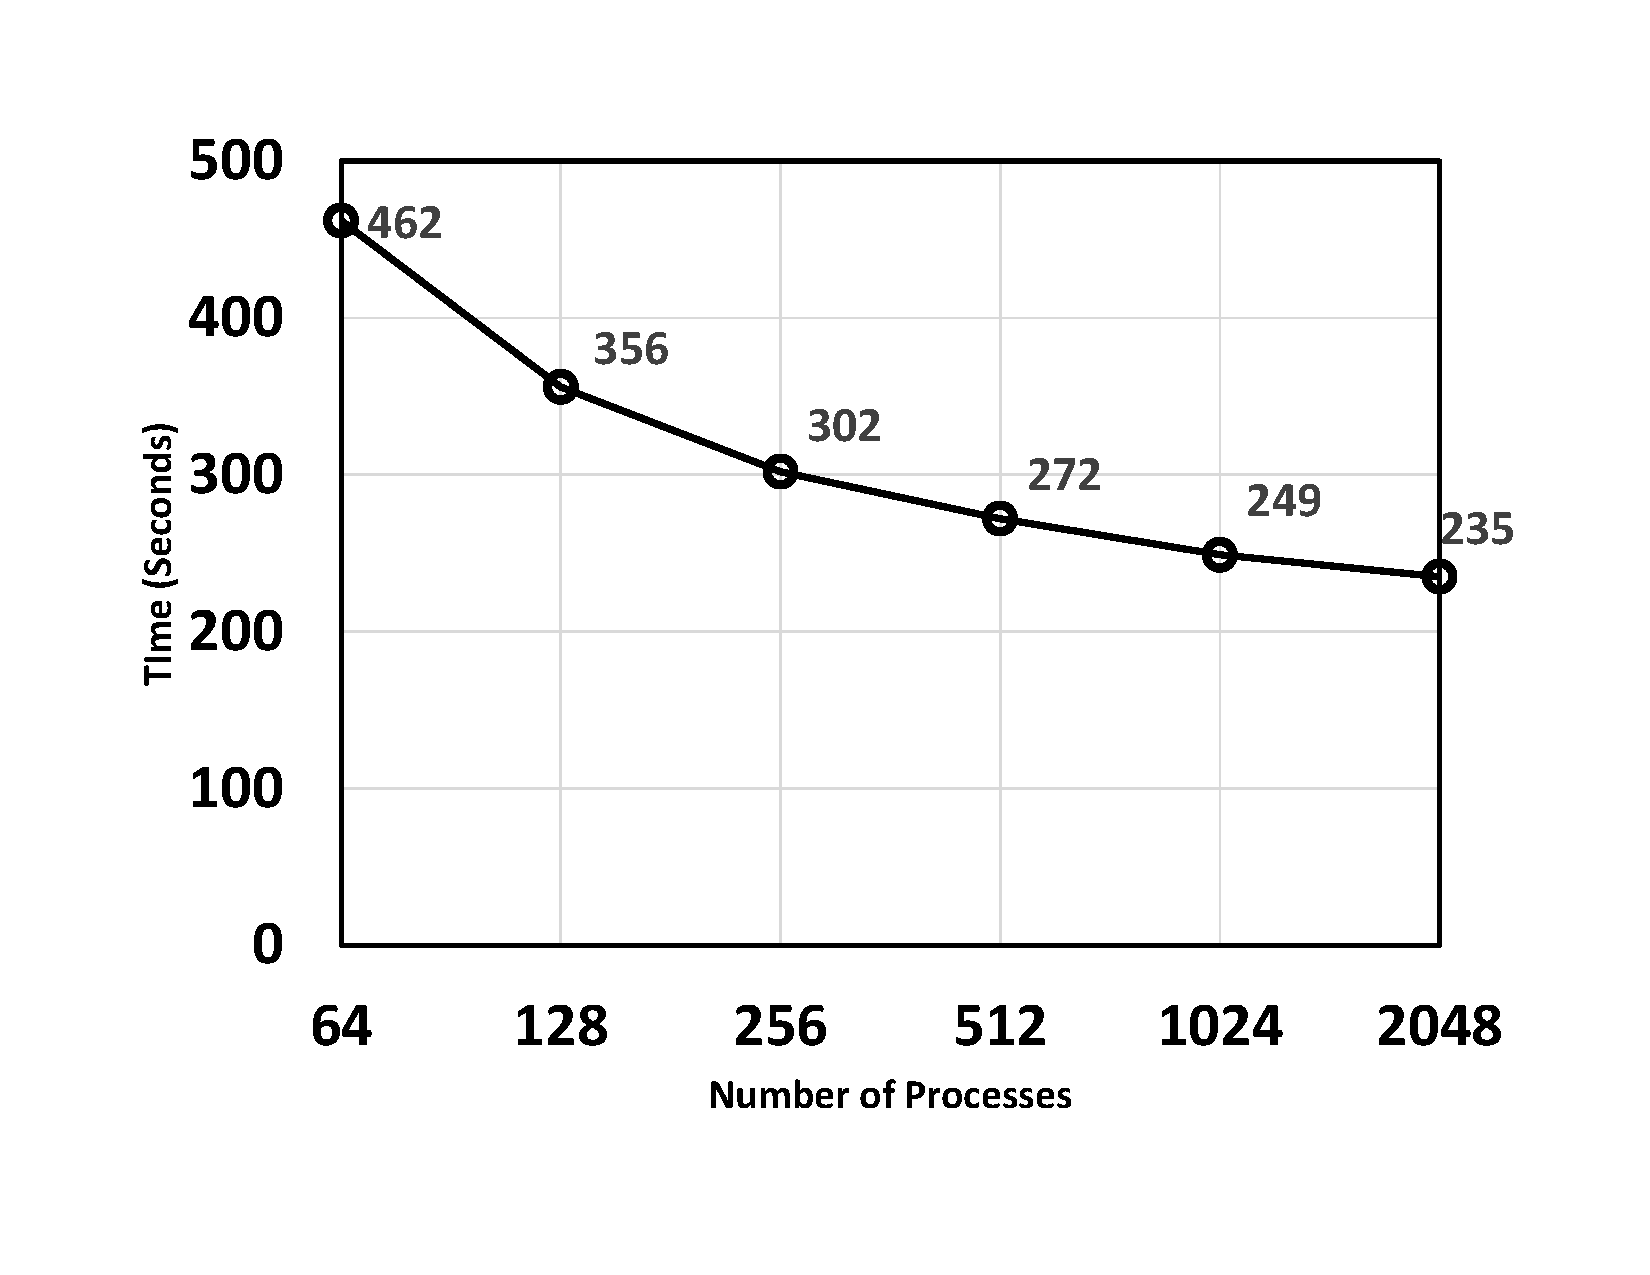
\includegraphics[trim = {25mm, 25mm, 25mm, 25mm}, width=.7\linewidth]{log/Strong_scaling.pdf}
	\caption{Strong-scaling results. \label{fig:strong_scale}}
\end{figure}
%
\begin{figure}
	\centering
	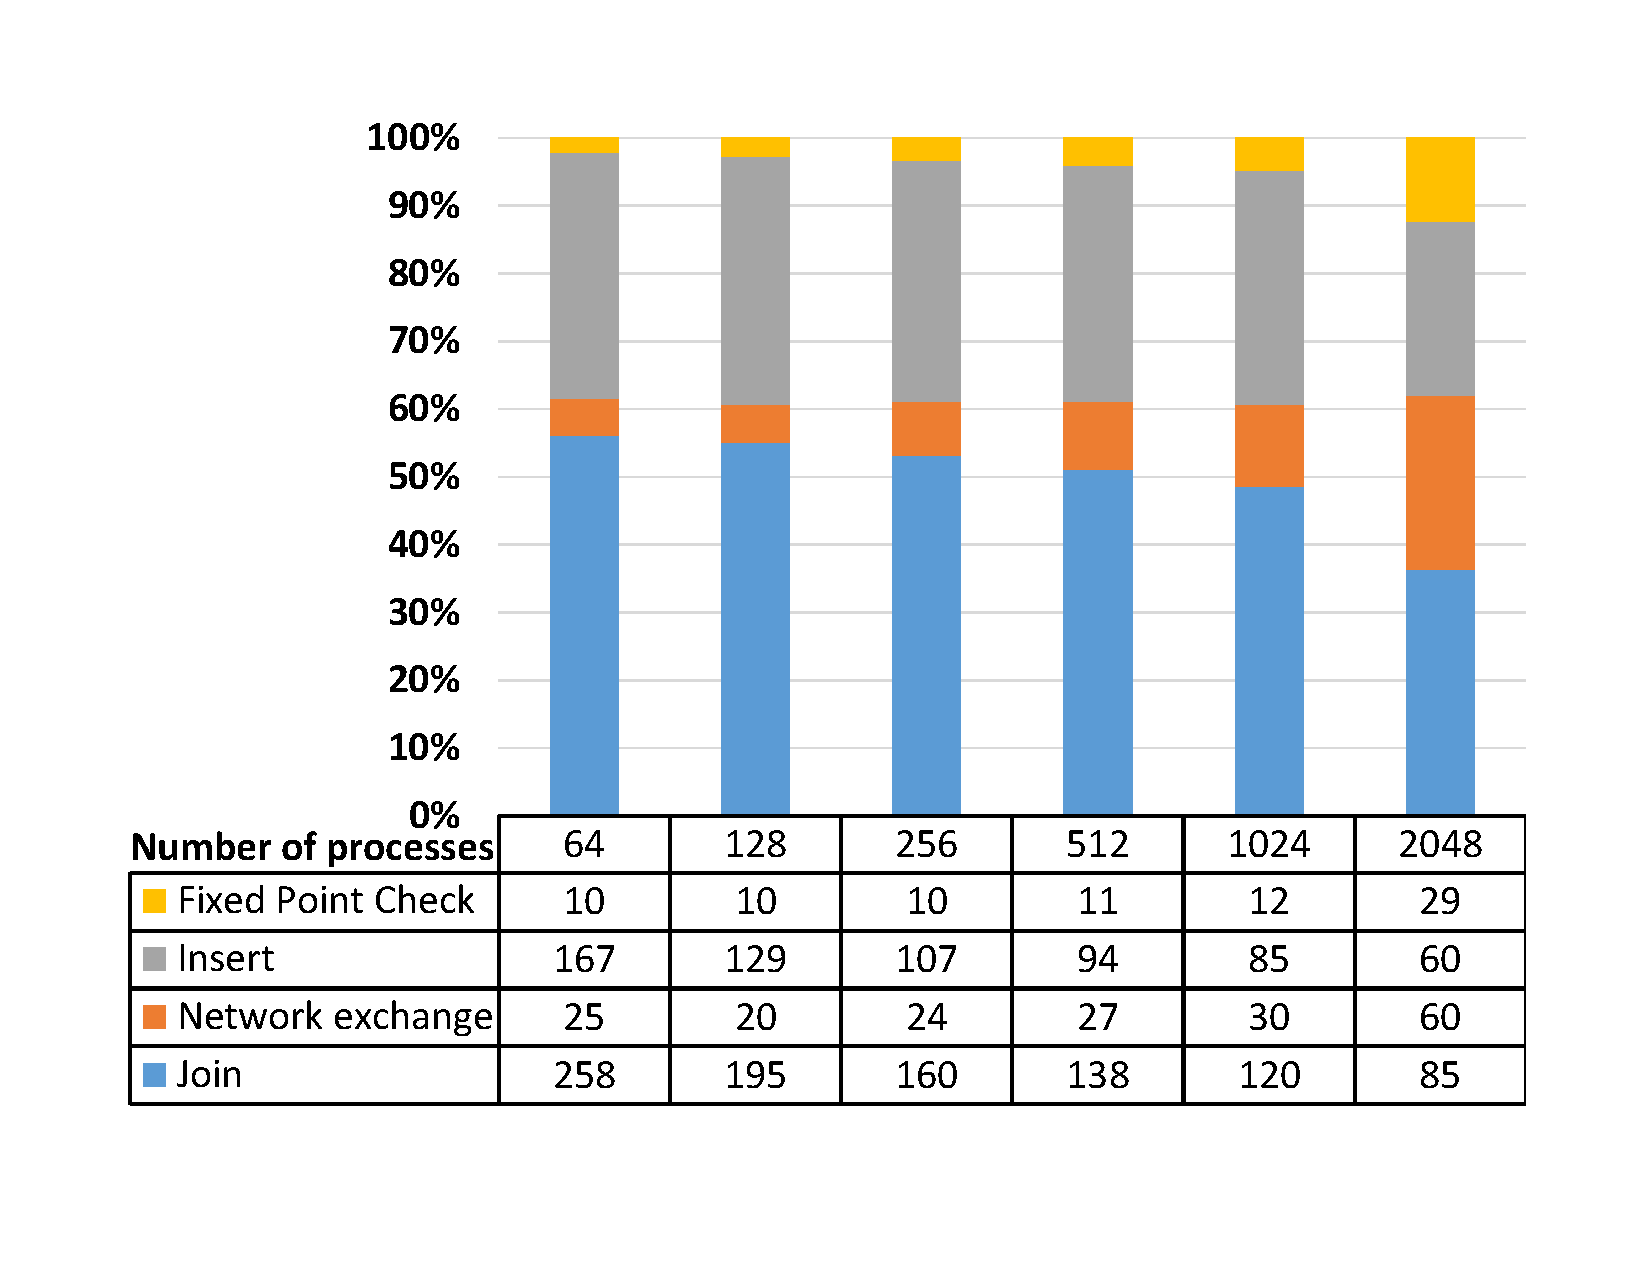
\includegraphics[trim = {25mm, 25mm, 25mm, 25mm}, width=.7\linewidth]{log/time_decomposition.pdf}
	\caption{Strong-scaling timing breakdown. \label{fig:decompose}}
\end{figure}


\subsection{Parallel Join}
%
Radix-hash join and merge-sort join are two of the most popularly used parallel implementations of the inner join operation.
Both these algorithms involve partitioning the input data so that they can be efficiently distributed 
to the participating processes. For example, in the radix-hash approach a tuple is assigned to a process 
based on the hash output of the column-value on which the join operation is keyed.
With this approach, tuples on both relations that share the same hash value
are always assigned to the same process. For every tuple in the left-hand side of the join relation is matched against all the tuples of the right-hand side of the join relation. Fast lookup data-structures like hash tables, or radix-trees (TRIE) can be used to organize the tuples within every process. The initial distribution of data using hashing reduces the overall computation overhead by a factor of the number of processes $(n)$. 

More recently ~\cite{Barthels:2017:DJA:3055540.3055545, Barthels:2015:RIJ:2723372.2750547}, there has been a concerted effort to implement JOIN operations on clusters using an MPI backend. The commonly used radix-hash join and merge-sort join have been re-designed for this purpose. 
Both these algorithms involve a hash-based partitioning of data so that they are be efficiently distributed 
to the participating processes and are designed such that inter-process communication is minimized. In both of these implementations
one-sided communication is used for transferring data between process. With one-sided communication the initiator of a data transfer request can directly access
parts of the remote memory and has full control where the data will be placed. Read and write operations are executed
without any involvement of the target machine. This approach of data transfer involves minimal synchronization between particiapting processes and have been shown to scale better that traditional two-sided communication. The implementation of parallel join has shown promising performance numbers; for example, the parallel join algorithm of~\cite{Barthels:2017:DJA:3055540.3055545}
ran successfully at 4,096 processor cores with up to 4.8 terabytes of input data.
%These results are very encouraging and we plan to extend our CFA pipeline to support MPI backend for processing datalog queries. To this end, we plan to extend the framework to work for relational operation kernels other than just the JOIN operation.


\subsection{Benchmarking: transitive closure}
%
Computing the transitive closure of a graph involves repeated join operations until a fixed point is reached.
We use the previously discussed radix-hash join algorithm to distribute the tuples across all processes.
The algorithm can then be roughly divided into four phases: 1) Join 2) network communication 3) insertion 4) checking for a fixed point.
In our join phase every process concurrently computes the join output of the local tuples. In the next phase every process sends the join output results to the relevant processes. This is a all-to-all communication phase, which we implemet using MPI's all\_to\_all routines. The next step involves inserting the join output result received from the network to the output graph's local partition. In the final step we check if the size of the output graph changed on any process, if it does then we have not yet reached a fixed point and we continue to another iteration of these 4 steps.


We performed a set of strong-scaling experiments to compute the transitive closure of graph with 412148 edges---the largest graph in the U. Florida Sparse Matrix set \cite{UF:SPMC}. We used the Quartz supercomputer at the Lawrence Livermore National Laboratory (LLNL). For our runs, we varied the number of processes from 64 to 2048. A fixed point was attained after 2933 iterations, with the resulting graph containing 1676697415 edges. As can be seen in Figure~\ref{fig:strong_scale}, our approach takes 462 seconds at 64 cores and 235 seconds at 2048 cores, corresponds to an overall efficiency of 6.25\%. We investigated these timings further by plotting the timing breakdown of by the four major components (join, network communication, join, fixed-point check) of the algorithm. We observe (see Figure~\ref{fig:decompose}) that for all our runs the total time is dominated by computation rather than communication; insert and join together tended to take up close to 90\% of the total time. This is quite an encouraging result  as it shows that we are not bound primarily by the network bandwidth (at these scales and likely moderately higher ones) and it gives us the opportunity to optimize the computation phase.

